149. \begin{figure}[ht!]
\center{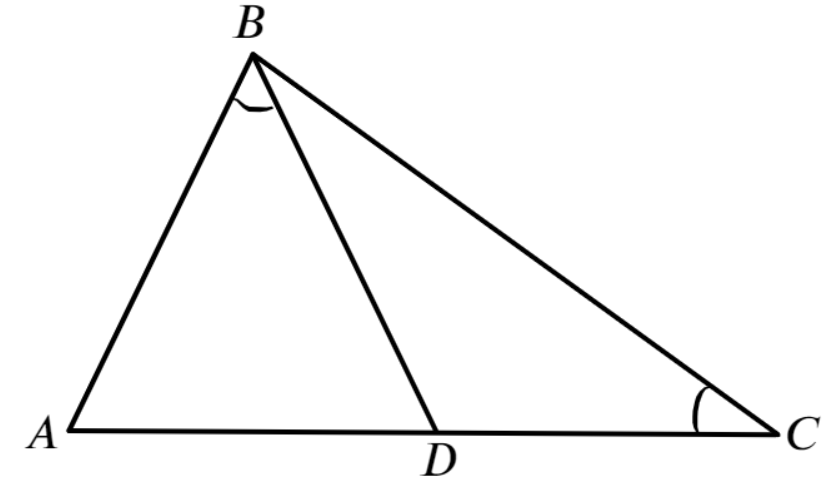
\includegraphics[scale=0.35]{g8-149.png}}
\end{figure}\\
Треугольники $ABD$ и $ABC$ подобны по двум углам ($\angle A$ --- общий, $\angle ABD=\angle C).$ Тогда $\cfrac{AD}{AB}=\cfrac{AB}{AC},\ \cfrac{AD}{2}=\cfrac{2}{4},$ значит $AD=1,\ DC=4-1=3.$\\
